\subsection{Panel zarządzania sklepem stacjonarnym}\label{subsec:panel-zarzadzania-sklepem-stacjonarnym}

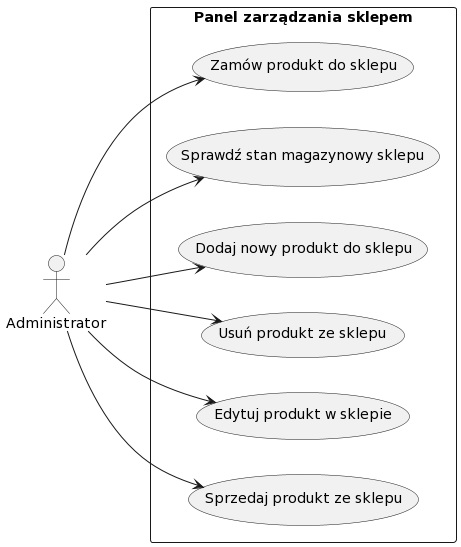
\includegraphics{../diagrams/use_cases/sklep}

\begin{enumerate}
\setcounter{enumi}{54}
\tightlist
\item
  {Zamów produkt do sklepu}
\end{enumerate}

{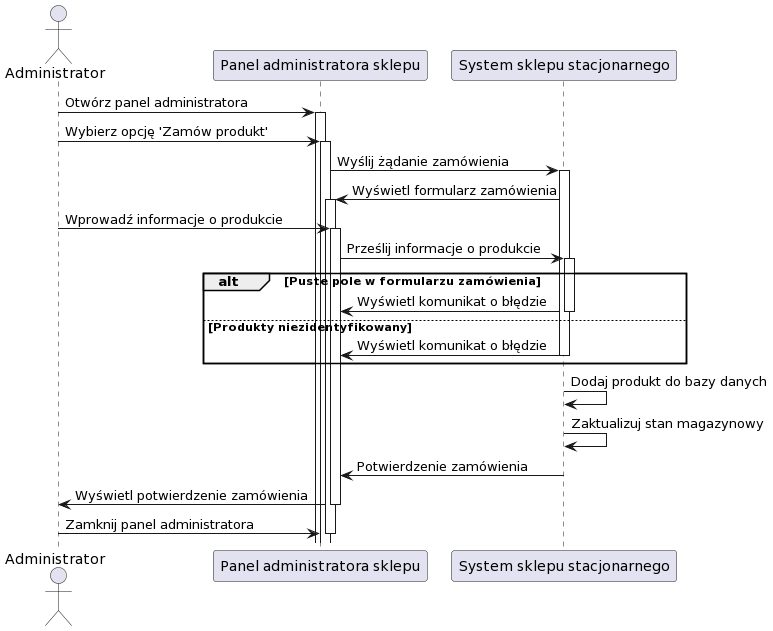
\includegraphics{../diagrams/sequence/sklep_zamow_produkt_do_sklepu}}

\item
{Aktorzy biorący udział: Administrator}

{Cel przypadku: Zamówienie produktu do sklepu stacjonarnego}

{Warunki początkowe: Administrator jest zalogowany do panelu
administratora sklepu stacjonarnego i posiada uprawnienia do dodawania
produktów.}

{Warunki końcowe: Nowy produkt zostaje dodany do bazy danych sklepu
stacjonarnego, liczba sztuk w magazynie zostaje zaktualizowana.}

{Główny ciąg zdarzeń:}

\begin{enumerate}
\tightlist
\item
  {Administrator otwiera panel administratora sklepu stacjonarnego.}
\item
  {Administrator wybiera opcję "Zamów produkt".}
\item
  {System wyświetla formularz zamówienia, który wymaga podania
  informacji o produkcie, takie jak nazwa, opis, cena i ilość.}
\item
  {Administrator wprowadza informacje o nowym produkcie i klika przycisk
  "Zamów".}
\item
  {System dodaje produkt do bazy danych sklepu stacjonarnego.}
\end{enumerate}

{Alternatywne ciągi zdarzeń:}

{4a. Administrator zostawia puste pole wymagane w formularzu
zamówienia.}

\begin{itemize}
\tightlist
\item
  {System wyświetla komunikat o błędzie i wymaga uzupełnienia pól
  wymaganych.}
\end{itemize}

{4b. Administrator wprowadza informacje o produkcie, którego nie ma w
bazie danych sklepu stacjonarnego.}

\begin{itemize}
\tightlist
\item
  {System wyświetla komunikat o błędzie i wymaga wprowadzenia innych
  informacji lub edycji istniejącego produktu.}
\end{itemize}

{}

\begin{enumerate}
\setcounter{enumi}{55}
\tightlist
\item
  {Sprawdź stan magazynowy sklepu}
\end{enumerate}

{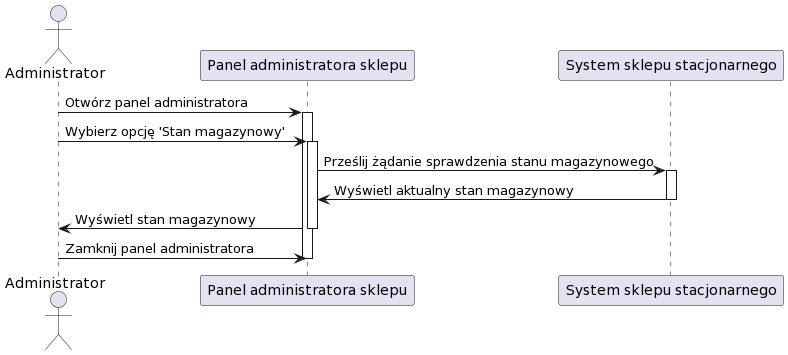
\includegraphics{../diagrams/sequence/sklep_sprawdz_stan_magazynowy}}

{Aktorzy biorący udział: Administrator}

{Cel przypadku: Sprawdzenie stanu magazynowego sklepu stacjonarnego}

{Warunki początkowe: Administrator jest zalogowany do panelu
administratora sklepu stacjonarnego i posiada uprawnienia do sprawdzania
stanu magazynowego.}

{Warunki końcowe: Administrator widzi aktualny stan magazynowy sklepu
stacjonarnego.}

{Główny ciąg zdarzeń:}

\begin{enumerate}
\tightlist
\item
  {Administrator otwiera panel administratora sklepu stacjonarnego.}
\item
  {Administrator wybiera opcję "Stan magazynowy".}
\item
  {System wyświetla aktualny stan magazynowy sklepu stacjonarnego.}
\end{enumerate}

{Alternatywne ciągi zdarzeń:}

{Brak alternatywnych ciągów zdarzeń.}

{}

\begin{enumerate}
\setcounter{enumi}{56}
\tightlist
\item
  {Dodaj nowy produkt do sklepu}
\end{enumerate}

{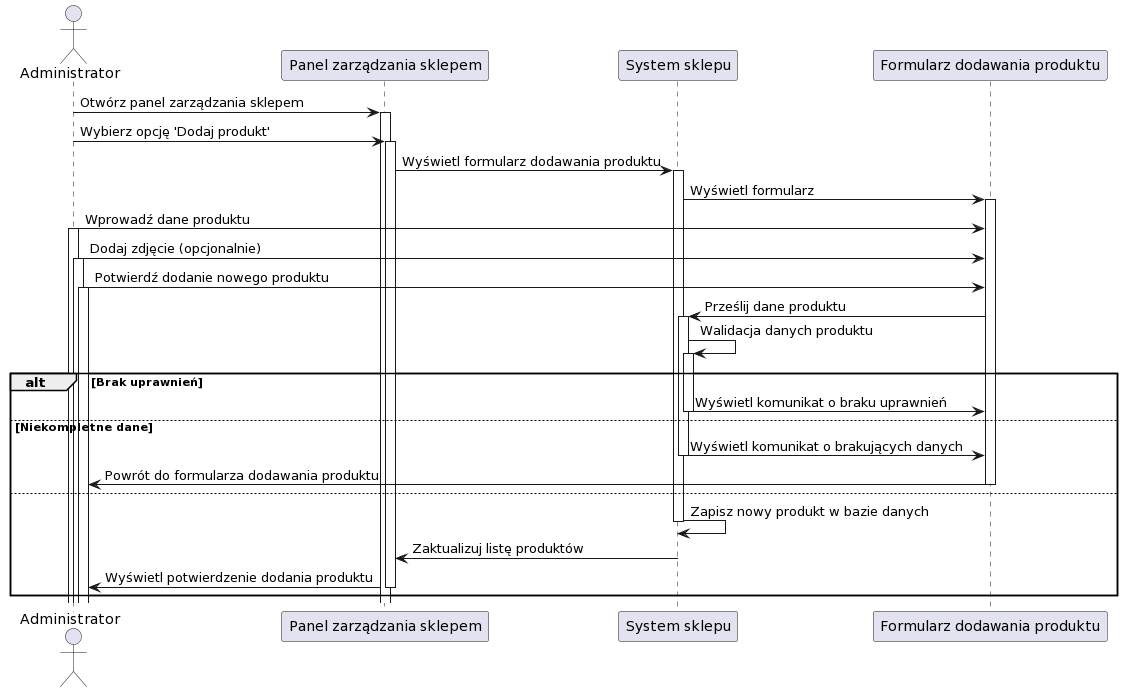
\includegraphics{../diagrams/sequence/sklep_dodaj_nowy_produkt}}

{Aktorzy biorący udział: Administrator}

{Cel przypadku: Dodanie nowego produktu do sklepu}

{Warunki początkowe: Administrator jest zalogowany do systemu i posiada
uprawnienia do dodawania nowych produktów.}

{Warunki końcowe: Nowy produkt zostaje dodany do sklepu i jest dostępny
dla klientów.}

{Główny ciąg zdarzeń:}

\begin{enumerate}
\tightlist
\item
  {Administrator otwiera panel zarządzania sklepem.}
\item
  {Administrator wybiera opcję "Dodaj produkt".}
\item
  {System wyświetla formularz dodawania produktu.}
\item
  {Administrator wprowadza nazwę, opis, cenę oraz ilość dostępnych sztuk
  nowego produktu.}
\item
  {Administrator dodaje zdjęcie produktu, jeśli jest to wymagane.}
\item
  {Administrator potwierdza dodanie nowego produktu do sklepu.}
\item
  {System zapisuje nowy produkt w bazie danych.}
\item
  {Nowy produkt jest widoczny w sklepie dla klientów.}
\end{enumerate}

{Alternatywne ciągi zdarzeń:}

\begin{itemize}
\tightlist
\item
  {W przypadku braku uprawnień, system wyświetla odpowiedni komunikat i
  nie pozwala na dodanie nowego produktu.}
\item
  {Jeśli któryś z wymaganych pól nie zostanie wypełniony, system
  wyświetla komunikat i zwraca użytkownika do formularza dodawania
  produktu, aby wprowadził brakujące dane.}
\end{itemize}

{}

\begin{enumerate}
\setcounter{enumi}{57}
\tightlist
\item
  {Usuń produkt ze sklepu}
\end{enumerate}

{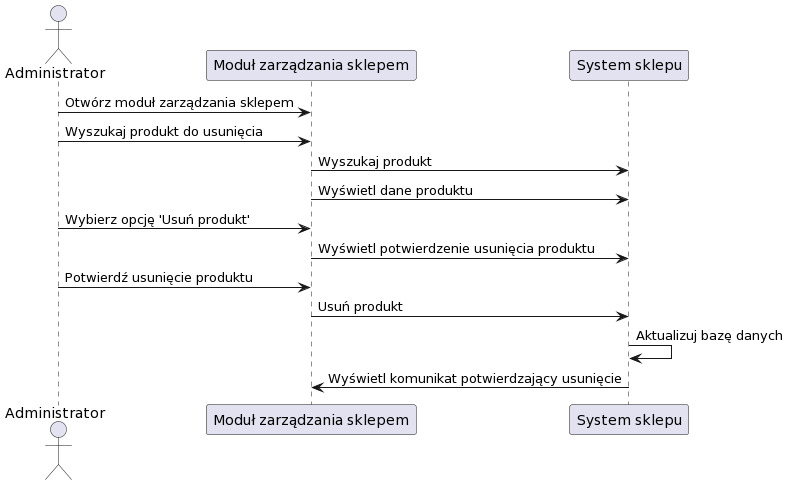
\includegraphics{../diagrams/sequence/sklep_usun_produkt_ze_sklepu}}

{Aktorzy biorący udział: Administrator}

{Cel przypadku: Usunięcie produktu ze sklepu}

{Warunki początkowe: Administrator jest zalogowany do systemu
zarządzania siłownią i posiada uprawnienia do usuwania produktów ze
sklepu.}

{Warunki końcowe: Produkt został usunięty ze sklepu.}

{Główny ciąg zdarzeń:}

\begin{enumerate}
\tightlist
\item
  {Administrator otwiera moduł zarządzania sklepem.}
\item
  {Administrator wyszukuje produkt, który chce usunąć.}
\item
  {Administrator wybiera opcję "Usuń produkt".}
\item
  {System wyświetla potwierdzenie usunięcia produktu.}
\item
  {Administrator potwierdza usunięcie produktu.}
\item
  {System usuwa produkt ze sklepu.}
\item
  {System wyświetla komunikat potwierdzający usunięcie produktu.}
\end{enumerate}

{Alternatywne ciągi zdarzeń:}

{5a. Jeśli administrator zrezygnuje z usunięcia produktu, system anuluje
proces usuwania i wraca do poprzedniego stanu.}

{}

{}

\begin{enumerate}
\setcounter{enumi}{58}
\tightlist
\item
  {Edytuj produkt w sklepie}
\end{enumerate}

{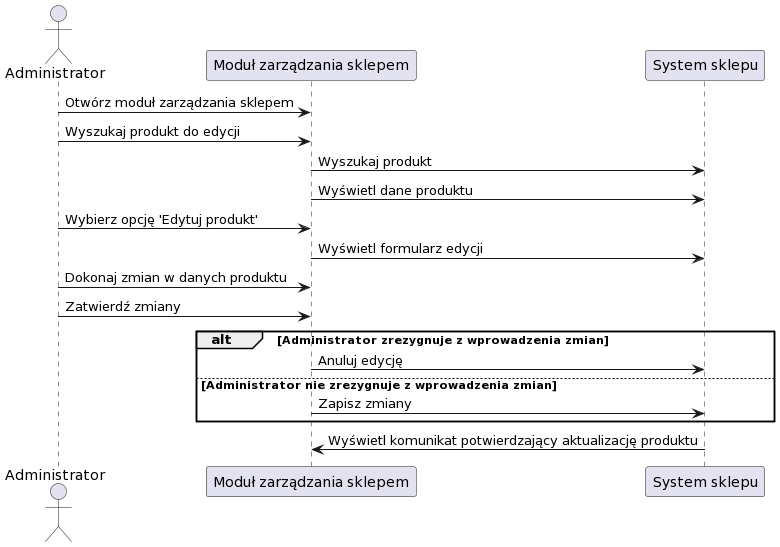
\includegraphics{../diagrams/sequence/sklep_edycja_produktu}}

{Aktorzy biorący udział: Administrator}

{Cel przypadku: Edycja produktu w sklepie}

{Warunki początkowe: Administrator jest zalogowany do systemu
zarządzania siłownią i posiada uprawnienia do edycji produktów w
sklepie.}

{Warunki końcowe: Produkt został zaktualizowany w sklepie.}

{Główny ciąg zdarzeń:}

\begin{enumerate}
\tightlist
\item
  {Administrator otwiera moduł zarządzania sklepem.}
\item
  {Administrator wyszukuje produkt, który chce edytować.}
\item
  {Administrator wybiera opcję "Edytuj produkt".}
\item
  {System wyświetla formularz edycji produktu.}
\item
  {Administrator dokonuje zmian w danych produktu.}
\item
  {Administrator zatwierdza zmiany.}
\item
  {System zapisuje zmiany w danych produktu.}
\item
  {System wyświetla komunikat potwierdzający aktualizację produktu.}
\end{enumerate}

{Alternatywne ciągi zdarzeń:}

{5a. Jeśli administrator zrezygnuje z wprowadzenia zmian, system anuluje
proces edycji i wraca do poprzedniego stanu.}

{}

\begin{enumerate}
\setcounter{enumi}{59}
\tightlist
\item
  {Sprzedaj produkt ze sklepu}
\end{enumerate}

{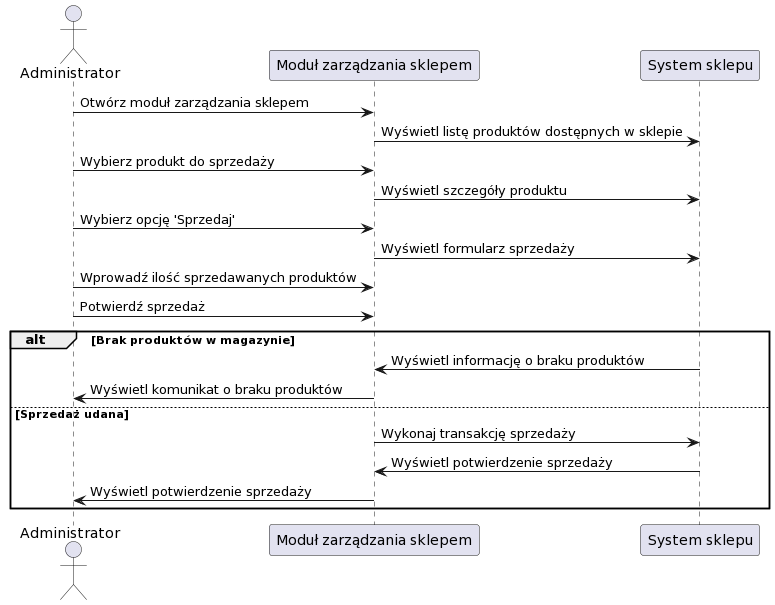
\includegraphics{../diagrams/sequence/sklep_sprzedaj_produkt}}

{Aktorzy biorący udział: Administrator}

{Cel przypadku: Dokonanie sprzedaży produktu ze sklepu stacjonarnego}

{Warunki początkowe: Administrator jest zalogowany do systemu i posiada
uprawnienia do sprzedaży produktów ze sklepu stacjonarnego. W sklepie
znajduje się co najmniej jeden produkt do sprzedania.}

{Warunki końcowe: zaktualizowanie stanu magazynowego produktu w
systemie.}

{Główny ciąg zdarzeń:}

\begin{enumerate}
\tightlist
\item
  {Administrator otwiera moduł zarządzania sklepem.}
\item
  {System wyświetla listę produktów dostępnych w sklepie stacjonarnym.}
\item
  {Administrator wybiera produkt, który chce sprzedać.}
\item
  {System wyświetla szczegóły wybranego produktu, takie jak nazwa, opis,
  cena, stan magazynowy.}
\item
  {Administrator wybiera opcję "Sprzedaj" przy wybranym produkcie.}
\item
  {System wyświetla formularz sprzedaży, w którym Administrator
  wprowadza ilość sprzedawanych produktów}
\item
  {Administrator potwierdza sprzedaż, klikając przycisk "Sprzedaj".}
\item
  {System wykonuje transakcję sprzedaży, aktualizując stan magazynowy
  produktu oraz generując potwierdzenie sprzedaży.}
\item
  {System wyświetla potwierdzenie sprzedaży wraz z informacjami o
  sprzedanym produkcie.}
\end{enumerate}

{Alternatywne ciągi zdarzeń:}

{1. Brak produktów w magazynie}

{System wyświetla informację o braku produktów w magazynie.}

{Administrator nie może dokonać sprzedaży i zamyka formularz sprzedaży.}

\begin{center}\rule{0.5\linewidth}{0.5pt}\end{center}

{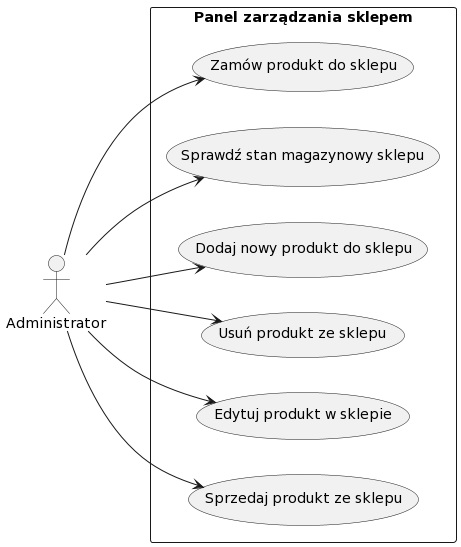
\includegraphics{../diagrams/use_cases/sklep}}
